% FieldElement51.as_bytes_spec: to_bytes is the bottleneck, and the harness
% fixes it drove.  One page (runs 09-21, 09-22, 09-24).
% Build: pdflatex as_bytes_to_bytes.tex
%        pdftoppm -png -r 300 as_bytes_to_bytes.pdf as_bytes
\documentclass[tikz,border=8pt]{standalone}
\usepackage[T1]{fontenc}
\usepackage{lmodern}
\renewcommand{\familydefault}{\sfdefault}
\usetikzlibrary{positioning,arrows.meta,calc}

\definecolor{agent}{RGB}{214,240,214}
\definecolor{agentline}{RGB}{60,140,60}
\definecolor{top}{RGB}{210,225,250}
\definecolor{topline}{RGB}{50,90,170}
\definecolor{fail}{RGB}{250,215,210}
\definecolor{failline}{RGB}{190,60,50}
\definecolor{todo}{RGB}{235,235,235}
\definecolor{todoline}{RGB}{140,140,140}

\tikzset{
  box/.style={draw, rounded corners=3pt, line width=0.9pt, align=center,
              minimum width=3.7cm, minimum height=1.3cm, inner sep=4pt},
  call/.style={-{Stealth[length=3mm]}, line width=1pt},
  prob/.style={draw=failline, fill=fail, rounded corners=3pt, line width=0.8pt,
               text width=7.9cm, minimum height=1.1cm, align=left, inner sep=5pt,
               font=\small},
  fix/.style={draw=agentline, fill=agent, rounded corners=3pt, line width=0.8pt,
              text width=7.9cm, minimum height=1.1cm, align=left, inner sep=5pt,
              font=\small},
}

\begin{document}
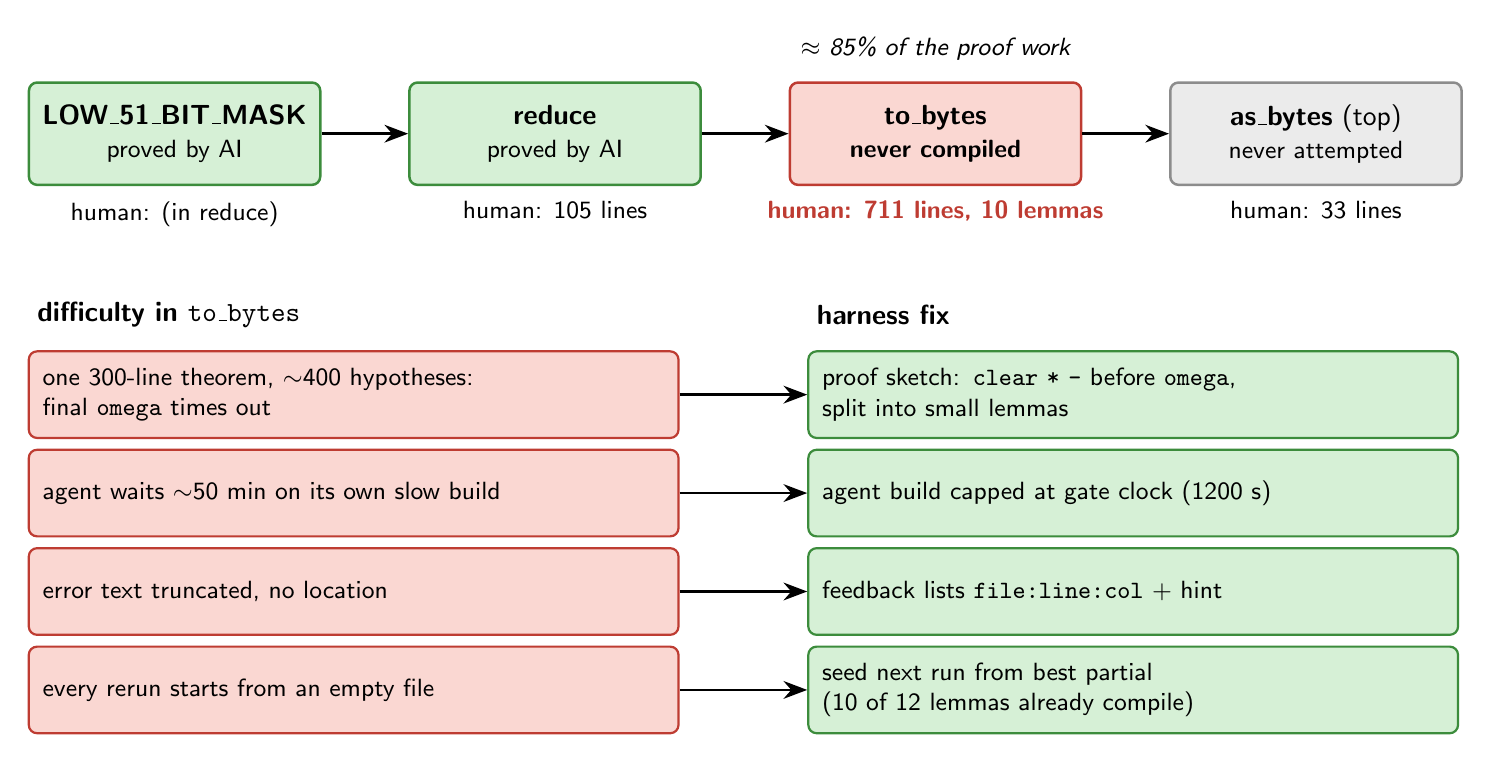
\begin{tikzpicture}[node distance=1.1cm]

  %% dependency chain, bottom-up = left to right
  \node[box, fill=agent, draw=agentline] (mk) {\textbf{LOW\_51\_BIT\_MASK}\\
    \small proved by AI};
  \node[box, fill=agent, draw=agentline, right=of mk] (rd) {\textbf{reduce}\\
    \small proved by AI};
  \node[box, fill=fail, draw=failline, right=of rd] (tb) {\textbf{to\_bytes}\\
    \small \textbf{never compiled}};
  \node[box, fill=todo, draw=todoline, right=of tb] (ab) {\textbf{as\_bytes} (top)\\
    \small never attempted};
  \draw[call] (mk) -- (rd);
  \draw[call] (rd) -- (tb);
  \draw[call] (tb) -- (ab);

  \node[font=\small, below=2pt of mk] {human: (in reduce)};
  \node[font=\small, below=2pt of rd] {human: 105 lines};
  \node[font=\small\bfseries, text=failline, below=2pt of tb] {human: 711 lines, 10 lemmas};
  \node[font=\small, below=2pt of ab] {human: 33 lines};

  \node[font=\small\itshape, above=4pt of tb] {$\approx$ 85\% of the proof work};

  %% difficulty -> fix
  \coordinate (L) at ($(mk.west)+(0,-2.3cm)$);
  \node[font=\bfseries, anchor=west] (hp) at (L) {difficulty in \texttt{to\_bytes}};
  \node[font=\bfseries, anchor=west] (hf) at ($(L)+(9.9cm,0)$) {harness fix};

  \foreach \i/\p/\f in {
      1/{one 300-line theorem, $\sim$400 hypotheses:\\ final \texttt{omega} times out}/
        {proof sketch: \texttt{clear * -} before \texttt{omega},\\ split into small lemmas},
      2/{agent waits $\sim$50 min on its own slow build}/
        {agent build capped at gate clock (1200 s)},
      3/{error text truncated, no location}/
        {feedback lists \texttt{file:line:col} + hint},
      4/{every rerun starts from an empty file}/
        {seed next run from best partial\\ (10 of 12 lemmas already compile)}} {
    \node[prob, anchor=north west] (p\i) at ($(L)+(0,-0.45cm-1.25cm*\i+1.25cm)$) {\p};
    \node[fix, anchor=north west]  (f\i) at ($(L)+(9.9cm,-0.45cm-1.25cm*\i+1.25cm)$) {\f};
    \draw[call] (p\i.east) -- (f\i.west);
  }
\end{tikzpicture}
\end{document}
